\chapter{The KZM across a first-order phase transition in a spin-1 BEC}


\section{Introduction}

\section{The Kibble-Zurek mechanism}
Consider a system that undergoes a spontaneous breaking of symmetry when a
control parameter, $\lambda$, is ramped across a phase transition that occurs
at the critical point, $\lambda_c$.
A continuous second-order phase transition can be characterized by a divergence
of the equilibrium correlation length
\begin{equation}
    \xi(\epsilon) = \frac{\xi_0}{|\epsilon|^z},
\end{equation}
and an equilibrium relaxation time
\begin{equation}
    \tau(\epsilon) = \frac{\tau_0}{|\epsilon|^{z\nu}},
    \label{eq:equil-relax-time}
\end{equation}
where
\begin{equation}
    \epsilon - \frac{\lambda_c - \lambda}{\lambda_c}
\end{equation}
is a reduced distance parameter.
The system is initially prepared in a high-symmetry phase $(\epsilon < 0)$ but 
breaks that symmetry as the critical point is crossed $(\epsilon > 0)$.
In the above equations, the exponents $z$ and $\nu$ are the dynamical and
correlation length critical exponents, respectively.
These exponents are determined by the universality class of the phase
transition, and different systems belonging to the same universality class share
the same critical exponents.
\textcolor{red}{Examples of different exponents for different classes? Links
to refs that calculate values?}
In contrast, the constants $\xi_0$ and $\tau_0$ are determined by the details
of the system. \par
The KZM describes the dynamics of crossing the critical point when $\lambda$ 
is continually varied.
We assume the form of a linear quench, such that the control parameter can be
written as
\begin{equation}
    \lambda(t) = \lambda_c - \epsilon(t),
\end{equation}
which is symmetric about the critical point so that the reduced distance
parameter is defined as
\begin{equation}
    \epsilon(t) = \frac{t}{\tau_Q}
    \label{eq:time-dependent-epsilon}
\end{equation}
for a quench time $\tau_Q$.
Here, $t \in [-\tau_Q, \tau_Q]$, where the critical point is reached at $t=0$.
From Eq.~\eqref{eq:equil-relax-time}, we see that far from the critical point
($|\lambda| \gg \lambda_c \implies |\epsilon| \gg 1$ ) the equilibrium
relaxation time is small compared to the time taken to reach the critical point
[Eq.~\eqref{eq:time-dependent-epsilon}]; which implies the dynamics is
adiabatic.
Conversely, as we approach the critical point ($\epsilon \rightarrow 0$), the
equilibrium relaxation time diverges and the dynamics of the system freeze,
known as critical slowing down.
As the critical point is passed, the system can once again resume the adiabatic
dynamics as the equilibrium relaxation time no longer diverges.
This then splits the dynamics into three parts as $\epsilon(t)$ is ramped from
$\epsilon(t) < 0 $ to $\epsilon(t) > 0$: adiabatic, frozen, and adiabatic again
(see Fig.~\ref{fig:adiabatic-impulse} for a schematic representation).
\begin{figure}
    \centering
    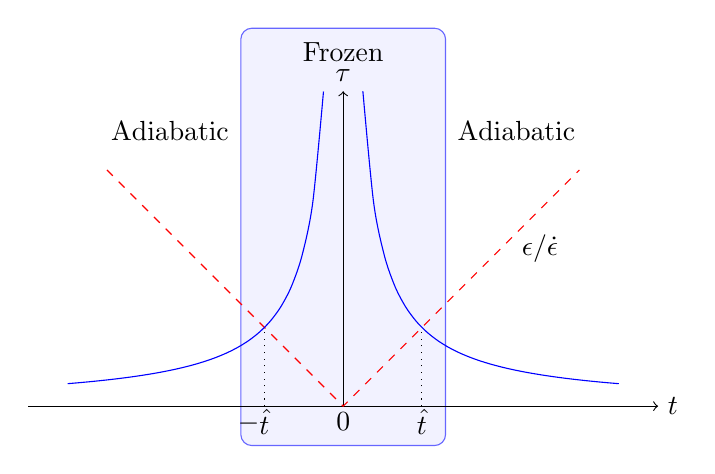
\begin{tikzpicture}
        \filldraw[color=blue!60, fill=blue!5, rounded corners] (-1.3, -0.5) 
        rectangle (1.3, 4.8);
        \draw[->] (-4, 0) -- (4, 0) node[right] {$t$};
        \draw[->] (0, 0) -- (0, 4) node[above] {$\tau$};
        \draw[scale=1, domain=-3:3, dashed, variable=\x, red] plot 
        ({\x}, {abs(\x)});
        \draw[scale=1, domain=0.25:3.5, smooth, variable=\x, blue] plot 
        ({\x}, {\x^(-1)});
        \draw[scale=1, domain=-3.5:-0.25, smooth, variable=\x, blue] plot 
        ({\x}, {abs(\x^(-1))});
        \node at (1, -0.2) {$\hat{t}$};
        \node at (-1, -0.2) {$\hat{t}$};
        \node at (-1.2, -0.22) {$-$};
        \draw[dotted] (1, 0) -- (1, 1);
        \draw[dotted] (-1, 0) -- (-1, 1);
        \node at (0, 4.5) {Frozen};
        \node at (2.5, 2) {$\epsilon/\dot{\epsilon}$};
        \node at (2.2, 3.5) {Adiabatic};
        \node at (-2.2, 3.5) {Adiabatic};
        \node at (0, -0.2) {$0$};
    \end{tikzpicture}
    \caption{A schematic representation of the dynamics of a system during a
    linear quench. The system starts in a high-symmetry phase ($t>0$) and is
    quenched across a critical point to a low symmetry phase ($t < 0$) by the
    reduced control parameter (red dashed line) $\epsilon(t)=t/\tau_q$. As
    the critical point is approached, the equilibrium relaxation time
    (blue line) diverges, and the order parameter can no longer follow the 
    ground state, leading to frozen dynamics in the interval
    $t \in [-\hat{t}, \hat{t}]$}
    \label{fig:adiabatic-impulse}
\end{figure}

The extent of the frozen region can be estimated by comparing the equilibrium
relaxation time with the time elapsed after the critical point
\begin{equation}
    \tau(t) \approx \left|\frac{\epsilon}{\dot{\epsilon}}\right|=t.
\end{equation}
Solving the above equation yields the freeze-out time $\hat{t}$:
\begin{equation}
    \hat{t} \sim (\tau_0\tau_Q^{z\nu})^{\frac{1}{1+z\nu}}.
\end{equation}
In the time interval $t \in [-\hat{t}, \hat{t}]$, the order parameter cannot
keep up with the change of the control parameter and therefore lags
behind the equilibrium value, $\hat{\epsilon}$, defined as
\begin{equation}
    \hat{\epsilon} \equiv |\epsilon(\hat{t})| \sim 
    \left(\frac{\tau_0}{\tau_Q}\right)^\frac{1}{1+z\nu}.
\end{equation}

As the symmetry of the system is broken, disconnected regions form which
have a spontaneously chosen value of the order parameter.
The size of these domains is set by the value of the equilibrium correlation
length at $\hat{t}$:
\begin{equation}
    \hat{\xi} \equiv \xi(\hat{t}) 
    = \xi_0 \left(\frac{\tau_Q}{\tau_0}\right)^\frac{\nu}{1 + z\nu}.
\end{equation}



\subsection{The generalized Kibble-Zurek mechanism}

\section{Broken-axisymmetry to ferromagnetic quench}

\subsection{Numerical set up}
\subsection{Scaling of FM domains}

\section{Bogoliubov analysis of the broken-axisymmetry phase}
\subsection{Calculating relevant modes}

\section{Other quench results? 2D?}
